
%%%%%%%%%%%%%%%%%%%%%%%%%%%%%%%%%%%%%%%%%%%%%%%%%%%%%%%%%%%%%%%%%%%%
% Related work
%%%%%%%%%%%%%%%%%%%%%%%%%%%%%%%%%%%%%%%%%%%%%%%%%%%%%%%%%%%%%%%%%%%%

%\vspace*{-2.0mm}
\section{Related Work}
\label{sec:related}


%%%%%%%%%%%%%%%%%%%%%%%%%%%%%%%%%%%%%%%%%
% 1. Connecting Parts in 3D Assemblies
%%%%%%%%%%%%%%%%%%%%%%%%%%%%%%%%%%%%%%%%%

\vspace*{2.0mm}
\noindent
{\bf Connecting Parts in 3D Assemblies.}  \
%Large and/or complex objects, such as architecture, are usually fabricated with parts rather than a single piece.
%This not only reduces the fabrication cost by using simpler parts, but also facilitate the maintenance since broken parts can be easily replaced \Mark{claim less about the maintenance; better to put it as a future work}.
To create a multi-part object for practical use,  component parts need to be assembled and tightly connected.
For example, glue is used to connect 3D printed parts~\cite{Chen-2015-Dapper,Vanek-2014-PackMerger, Hu-2014-Pyramidal}
although glued parts cannot be separated easily, discouraging parts disassembly and reassembly.
% and its connection strength is highly dependent on the part material.
Nails and screws are commonly used in furniture~\cite{Shao-2016-Furniture,Lau-2011-Furniture}.
% and laser-cut objects~\cite{Weichel-2012-Enclosed}.
However, these fasteners may break the parts and become loose after repeated disassembly and reassembly.
Wire also can be used for  part connections~\cite{Attene-2015-ShapesInABox, Richter-2015-BeamMeshes}, yet tying parts together could be a tedious task.

\begin{figure}[!b]
	\centering
	\vspace*{-4.0mm}
	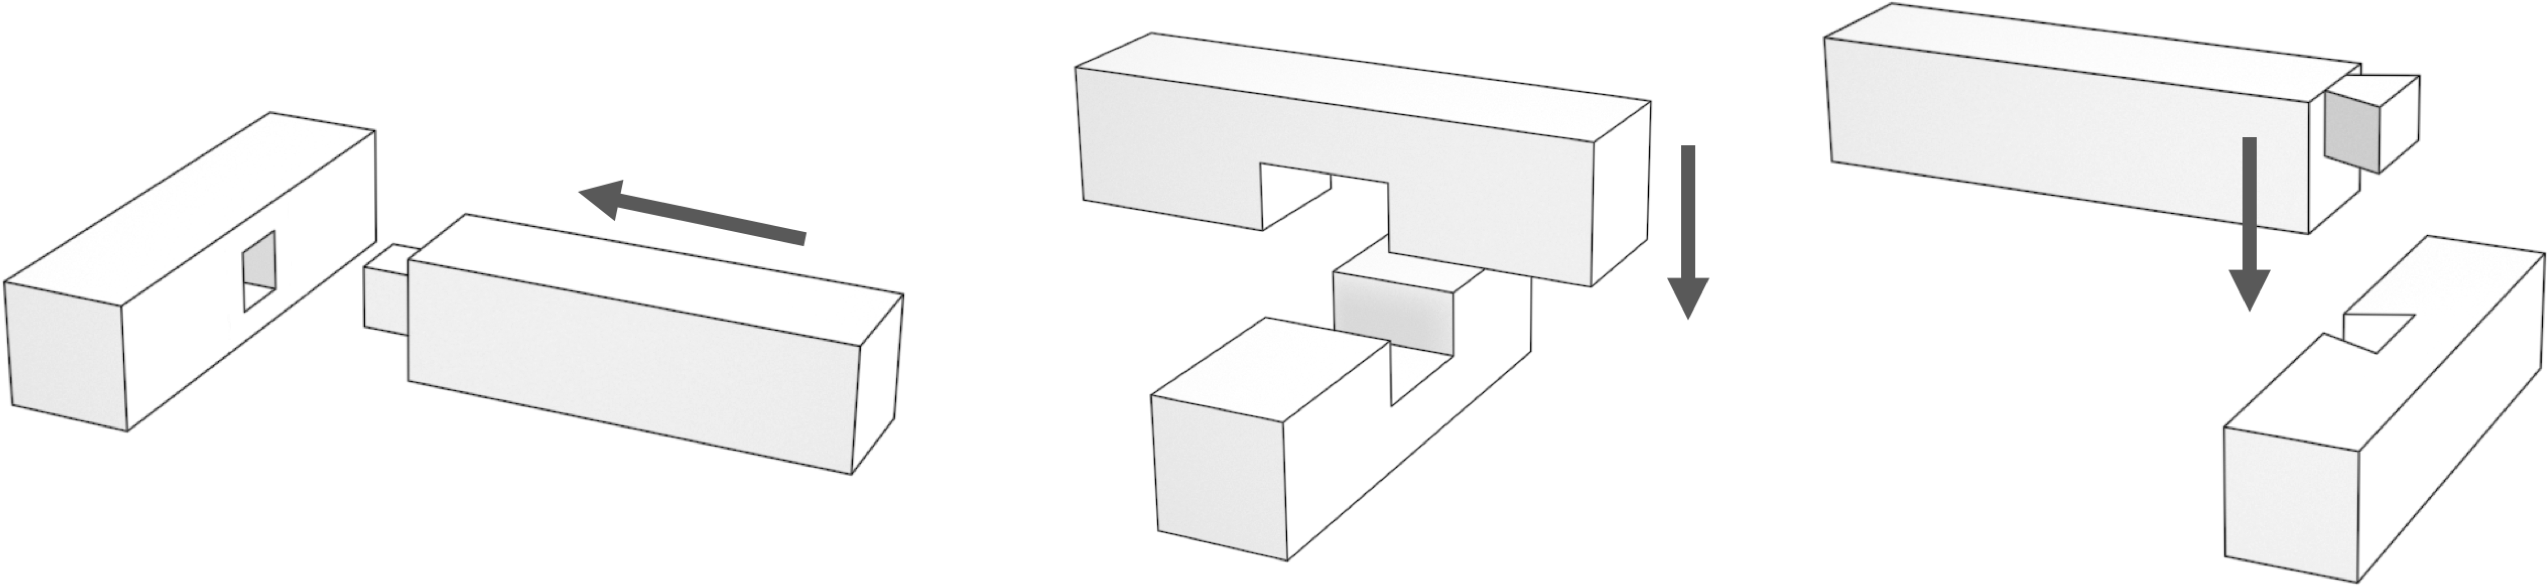
\includegraphics[width=8.00cm]{images/Joints.png}
	\vspace*{-2.5mm}
	\caption{Example woodworking joints. From left to right: mortise-and-tenon, halved joint, and dovetail joint, where the black arrow shows the single part movable direction allowed by the joint.}
	%\vspace*{-4.0mm}
	\label{fig:Joints}
\end{figure}


In practice, integral joints are often preferred for connecting parts, since they greatly simplify the assembly process. For example, woodworking joints (see Figure~\ref{fig:Joints}) are widely used in furniture design~\cite{Yao-2017-DecorativeJoinery,Koo-2017-ZeroWaste,Chen-2015-FreshPressModeler,Schwartzburg-2013-PlanarPieces},
mortise-and-tenon joints for 3D printed object assemblies~\cite{Luo-2012-Chopper, Hao-2011-PartitionModels, Duncan-2016-Hands-OnAssembly}, and
halved joints for laser-cut shape abstractions~\cite{Cignoni-2014-MeshJoinery,  Hildebrand-2012-crdbrd,McCrae-2011-Slices}.
However, these joints only constrain relative part motion locally, and the resulting assembly typically relies on other means, e.g., friction and/or gravity, to lock the parts in place.
%\Mark{add a figure to show various parts connection methods}

%%%%%%%%%%%%%%%%%%%%%%%%%%%%%%%%%%%%%%%%%
% 2. Self-supporting Structures
%%%%%%%%%%%%%%%%%%%%%%%%%%%%%%%%%%%%%%%%%

\vspace*{2.0mm}
\noindent
{\bf Self-supporting Structures},  
e.g., masonry buildings~\cite{Rippmann-2016-ArmadilloVault} and puzzles~\cite{Frick-2015-Self-SupportPuzzle}, are assemblies of rigid components that do not require any binder to connect the parts. The entire structure is in static equilibrium through gravity-induced compression forces that immobilize all the parts~\cite{Whiting-2009-ModelMasonry}.
%
Recently, the design of freeform self-supporting structures has  received a lot of interest in computer graphics.
Some research works focus on designing 3D surfaces that only exhibit internal compression forces under gravity~\cite{Miki-2015-AiryStressFunctions,Tang-2014-PolyhedralMesh,Liu-2013-RegularTriangulation,deGoes-2013-Equilibrium,Vouga-2012-Self-SupportSurface},
while others focus on the design, fabrication, and assembly of self-supporting structures~\cite{Rippmann-2016-ArmadilloVault,Deuss-2014-AssembleSelfSupport,Panozzo-2013-SelfSupportMasonry}.  
%
Self-supporting structures can only bear compression load but are not designed to handle any tensile forces.
This is reasonable for certain architectural structures that are built to bear their own weight, but not for general spatial assemblies that experience forces in arbitrary directions. The strategy of immobilizing parts in self-supporting structures is therefore not applicable in our general assembly setting.

%In particular, Panozzo et al.~\shortcite{Panozzo-2013-SelfSupportMasonry} designed and fabricated unreinforced masonry models consisting of hexagonal blocks while
%Deuss et al.~\shortcite{Deuss-2014-AssembleSelfSupport} constructed freeform self-supporting structures by using a sparse set of chains connected to fixed anchor points.




%%%%%%%%%%%%%%%%%%%%%%%%%%%%%%%%%%%%%%%%%
% 3. Interlocking Assemblies
%%%%%%%%%%%%%%%%%%%%%%%%%%%%%%%%%%%%%%%%%

\vspace*{2.0mm}
\noindent
{\bf Interlocking Assemblies.} \ 
Several computational methods have recently been developed to construct interlocking assemblies. 
Xin et al.~\shortcite{Xin-2011-BurrPuzzles} create 3D interlocking puzzles by replicating and connecting multiple instances of a six-piece interlocking burr structure. 
Rather than reusing an existing structure,  Song et al. ~\shortcite{Song-2012-InterCubes} construct 3D interlocking
puzzles by iteratively extracting pieces from a voxelized 3D shape and enforcing a local interlocking condition among every three consecutive pieces. 
Song et al.~\shortcite{Song-2015-Interlock} extend this method to handle smooth non-voxelized shapes for 3D printing.
Zhang and Balkcom~\shortcite{Zhang-2016-InterlockVoxel} define a set of voxel-like interlocking blocks and connect instances of these blocks layer-by-layer into various voxelized shapes. 

Different from above works that take a 3D solid object as an input, Fu et al.~\shortcite{Fu-2015-Furniture} focus on frame-based structures such as furniture that have been initially partitioned into parts. They compute an interlocking joint configuration by planning and connecting local interlocking groups.
This method has been extended to interlock 2D laser-cut parts into a convex polyhedron~\cite{Song-2016-CoFiFab} and to design reconfigurable furniture with multi-key interlocking~\cite{Song-2017-ReconfigInterlock}.
Yao et al.~\shortcite{Yao-2017-InterlockShell} design and optimize interlocking shell pieces for 3D printing. They employ 3D simulation to test whether the resulting shell assemblies are interlocking.
However, this generate-and-test paradigm is relatively inefficient and applicable only for assemblies with a small number of interlocking pieces.

The key idea of the above works (except~\cite{Yao-2017-InterlockShell}) is to design interlocking assemblies by constructing and connecting multiple local interlocking groups.  
This strategy skillfully avoids the global test for interlocking of the resulting assemblies, which would have a time complexity that is exponential in the number of parts~\cite{Song-2012-InterCubes}. 
While this strategy allows designing interlocking assemblies with many parts, the search space is restricted to a small subset of all possible interlocking configurations.
Our experimental results in Section~\ref{sec:results}  show that the flexibility of designing interlocking assemblies can be significantly increased by our method's ability to explore the full search space.
%indicate that this restricted subset is indeed very small, and
%\Mark{need to show why the small subset is not good or to show the goodness of interlocking configurations that are out of the subset.}

\if 0
Compared with above works that focus on each specific kind of interlocking assemblies, this work studies the common governing mechanics of interlocking assemblies that may have different forms and develops a general constructive approach for designing these assemblies.
In particular, this work builds connections between interlocking assemblies and the NDBG~\cite{Wilson-1992-AssemblyPlanning}, making it possible to take advantage of existing graph theory and algorithms to explore the full search space of interlocking configurations. 
%This not only leads to an approach that can test interlocking with polynomial time complexity, 
\fi



%%%%%%%%%%%%%%%%%%%%%%%%%%%%%%%%%%%%%%%%%
% 4. Assembly Planning
%%%%%%%%%%%%%%%%%%%%%%%%%%%%%%%%%%%%%%%%%

\vspace*{2.0mm}
\noindent
{\bf Assembly Planning} \
is the problem of finding a sequence of motions to assemble a structure from its parts. 
This problem has been extensively studied in robotics and we refer to~\cite{Ghandi-2015-AssemblyPlanningReview} for a thorough review.
Assembly planning is also relevant for computer graphics applications, e.g., for generating visual assembly instructions~\cite{Agrawala-2003-AssemblyInstructions,Guo-2013-IllustrateDisassembly} or creating exploded view diagrams~\cite{Li-2008-ExplodedView}.

Finding an assembly plan requires identifying movable parts and part groups at each stage of the assembly, often leading to a combinatorial search problem.
To solve this task more efficiently, Wilson~\shortcite{Wilson-1992-AssemblyPlanning} invented a {\em Directional Blocking Graph} and a {\em Non-Directional Blocking Graph} to represent blocking relations among parts in an assembly. 
Tai~\shortcite{Tai-2012-InterlockRF} employed these graphs for designing reciprocal frames connected with notched joints, aiming at minimizing the number of movable parts and part groups in the final assembly.
%\Mark{good to cite some works outside of computer graphics community;
%	we focus on designing parts geometry while above works focus on "designing" (dis)assembly sequences }
Rather than focusing on assembly planning, our work, to the best of our knowledge, is the first to employ these graphs for computational design of interlocking assemblies. 
% parts and/or joints geometry construction for designing new interlocking assemblies.




\if 0
, Wilson and Latombe~\shortcite{Wilson-1994-GeometricReasoning} developed a {\em Directional Blocking Graph} (DBG)  to represent blocking relations among parts in an assembly along a certain translational direction and summarized all these graphs for all possible translational directions to construct a {\em non-directional blocking graph} (NDBG).
The NDBG allows to address the combinatorial problem of automatically computing the assembly sequences of a 3D assembly in polynomial time complexity of the number of parts involved. 
Tai~\shortcite{Tai-2012-InterlockRF}  presented a computational approach to construct wooden frames connected with notched joints.
They search  joint configurations using a  genetic algorithm to find wooden frame that is disassemblable and leans towards being global interlocking.
Directional Blocking Graph (DBG) is employed to identify all movable parts or part groups in the assembly to analyze the interlocking condition.
\fi





%\newpage







%%%%%%%%%%%%%%%%%%%%%%%%%%%%%%%%%%%%%%%%%%%%%%%%%%%%%%%%%%%%%%%%%%%%%%%%%%%%%%
% Backup
%%%%%%%%%%%%%%%%%%%%%%%%%%%%%%%%%%%%%%%%%%%%%%%%%%%%%%%%%%%%%%%%%%%%%%%%%%%%%%





